\documentclass[12pt]{article}

\usepackage[utf8]{inputenc}
\usepackage[T1]{fontenc}

% clickable links in pdf
\usepackage{hyperref}

% make title variable available
\usepackage{titling}

% create own header footer
\usepackage{fancyhdr}

% images
\usepackage{graphicx}

% grafics powerfull and hard
\usepackage{tikz}

% character spacing to fill line
\usepackage{microtype}

% image placement with [H]
\usepackage{float}

% fancy quotes
\usepackage{epigraph}

% extra symbols
\usepackage{textcomp}

% display code
\usepackage{listings}

% icons
\usepackage{fontawesome}

% set dimmensions of page
\usepackage[footskip=80pt, headheight=15pt]{geometry}

% tables
\usepackage{tabularx}
\usepackage{makecell}

% make code copyable
\lstset{
upquote=true,
columns=fullflexible,
literate={*}{{\char42}}1
         {-}{{\char45}}1
}

\newsavebox{\picbox}

\graphicspath{ {./images/} }

% command for rounded corners
\newcommand{\cutpic}[3]{
  \savebox{\picbox}{\includegraphics[width=#2]{#3}}
  \tikz\node [draw, rounded corners=#1, line width=4pt,
    color=white, minimum width=\wd\picbox,
    minimum height=\ht\picbox, path picture={
      \node at (path picture bounding box.center) {
        \usebox{\picbox}};
    }] {};}

\newcommand{\requirementTable}[5]{
    \begin{table}[H]
      \begin{tabularx}{\textwidth}{|l|X|}
        \hline
        Bezeichnung & #1  \\ \hline
        Akteur (= Auslöser) & #2  \\ \hline
        Voraussetzung & #3  \\ \hline
        Funktionsablauf & #4  \\ \hline
        Endzustand & #5  \\ \hline
      \end{tabularx}
    \end{table}
}

\title{
  \Huge
  \textbf{Globalizer} \\
  \vspace{0.2cm}
  \LARGE
  Anforderungsspezifikationen
}

\date{27.09.2018}

\author{
  Koller, Jonas\\
  \texttt{jonas.koller@gmx.ch} \\
  Wolfisberg, Donato \\
  \texttt{donato.wolfisberg@gmail.com}
}

\pagestyle{fancy}
\fancyhf{}
\lhead{BBZW Sursee Rötheli Manfred}
\rhead{Globalizer Anforderungsspezifikationen}
\lfoot{Jonas Koller \& \\ Donato Wolfisberg}
\cfoot{\thedate}
\rfoot{\thepage}

\renewcommand{\headrulewidth}{1pt}
\renewcommand{\footrulewidth}{1pt}

\renewcommand{\contentsname}{Inhalt}

\begin{document}
  \begin{titlepage}
    \pagenumbering{gobble}

    \begin{center}
      \vspace*{-2cm}
      \cutpic{0.8cm}{4cm}{logo.jpg}

      \thetitle

      \vspace{2cm}

      \textbf{\theauthor}

      \vspace{1.5cm}

      \thedate
    \end{center}

    \vfill

    \begin{figure}[H]
        \makebox[\linewidth]{
            
\includegraphics[width=1.3\linewidth]{globe.jpg}
        }
        \vspace*{-5cm}
    \end{figure}
  \end{titlepage}

  \newpage
  \pagenumbering{Roman}

  \begin{center}
    \makebox[\textwidth]{
\includegraphics[width=\paperwidth]{nightsky.jpg}}
  \end{center}

  \section{Zweck des Dokuments}
    In diesem Dokument werden wir die Anforderungen an unser Projekt “Globalizer” formulieren. Das Projekt gilt im aktuellen Zustand als angenommen, da der Projektantrag durch Herr Manfred Rötheli angenommen wurde. Wir werden beschreiben, welche Anforderungen wir erfüllen möchten (“soll”-Anforderungen) und welche optionalen “kann”-Anforderungen wir eventuell auch erfüllen können. Es soll eine Übersicht für unser Vorhaben sein. Weiter sollen unsere Prozesse so gut wie möglich durch Grafiken dargestellt und visualisiert werden. \\
    Bei Fragen wenden sie sich an den Projektleiter (jonas.koller@gmx.ch).

  \section{Allgemeine Informationen}
    Hier folgt eine kurze Auflistung der Informationen zu diesem Dokument, dem Entwicklungsteam und dem aktuellen Stand.

  \subsection{Projektmitarbeiter}
    \begin{table}[h]
      \begin{tabularx}{\textwidth}{|l|l|X|l|}
        \hline
        \textbf{Name} & \textbf{Vorname}  & \textbf{E-Mail}                & \textbf{Funktion}     \\ \hline
        Koller        & Jonas             & jonas.koller@gmx.ch            & Projektleiter         \\ \hline
        Wolfisberg    & Donato            & donato.wolfisberg@gmail.com    & Entwickler            \\ \hline
        Gian          & Ott               & gian\_ott@sluz.ch              & Prüfer                \\ \hline
        Manuel        & Troxler           & manuel\_troxler@sluz.ch        & Prüfer                \\ \hline
      \end{tabularx}%
    \end{table}

  \subsection{Änderungskontrolle}
    \begin{table}[h]
      \begin{tabularx}{\textwidth}{|l|l|l|X|}
        \hline
        \textbf{Version} & \textbf{Datum} & \textbf{Ausführende Stelle} & \textbf{Bemerkung}                     \\ \hline
        1                & 21.09.2018     & Projektteam                 & \makecell[l]{Erste Version des Dokuments \\ erstellt}  \\
        2                & 23.09.2018     & Projektteam                 & \makecell[l]{Gesamtüberblick erstellt}  \\
        3                & 25.09.2018     & Projektteam                 & \makecell[l]{Zielkatalog erstellt}  \\
        4                & 27.09.2018     & Projektteam                 & \makecell[l]{Abschliessende Arbeiten}  \\
        \hline
      \end{tabularx}
    \end{table}

  \subsection{Prüfung}
    \begin{table}[h]
      \begin{tabularx}{\textwidth}{|l|l|X|}
        \hline
        \textbf{Version} & \textbf{Datum} & \textbf{Ausführende Stelle}     \\ \hline
        4                 & 27.09.2018    & Gian Ott                        \\ \hline
      \end{tabularx}
    \end{table}

  \newpage
  \tableofcontents
  \newpage

  \pagenumbering{arabic}


  \section{Gesamtüberblick}
    \subsection{Allgemeine Beschreibung}
        Der Auftraggeber gehört zum Berufsbildungszentrum Wirtschaft, Informatik und Technik (BBZW) des Kanton Luzern, das Kompetenzzentrum für kaufmännische und gewerbliche Berufe an den drei Schulstandorten Sursee, Willisau und Emmen. Am Standort Sursee werden die zukünftigen Informatiker EFZ ausgebildet. \\
        Der eigentliche Auftraggeber ist  die Schule BBZW Sursee. Sie will eine Chat Applikation entwickeln lassen für die Kommunikation unter den Schülern wie auch zum Lehrer. Es ist ihm wichtig, dass die Anwender der Applikation komplett anonym bleiben können. Die Applikation soll modern und schnell als Webseite daher kommen und sowohl im Browser als auch auf mobilen Geräten funktionieren. \\
        Das Resultat soll auch ausserhalb der Organisation gezeigt werden können, damit die Kompetenz des BBZW Sursee auch dort sichtbar wird.
        Der Auftraggeber möchte auch den Open-source-Ansatz fördern. Darum soll das Projekt unter open-source durchgeführt werden und der Auftraggeber übernimmt die Verantwortung für Koordination und die Projektleitung, alle anderen Arbeiten müssen durch motivierte Freiwillige geleistet werden. \\
        Finanziell kann sich der Auftraggeber und der Kanton Luzern als Inhaber nichts leisten. Darum muss das Projekt mit einem minimalen Budget auskommen.

    \subsection{Ziele}
      Die Chat Applikation soll die folgende Eigenschaften haben.

      \begin{enumerate}
        \item Modernes Design: Das Ziel besteht aus jungen Menschen, die gewohnt sind, mit Informatik Instrumenten arbeiten. Das erhöht die Akzeptanz der Anwendung. Da die Anwendung auch ausserhalb des BBZW gezeigt werden soll, ist das sehr wichtig für das Bild, welches die anderen vom BBZW bekommen.
        \item Anonymität der Anwender:  Im Moment sind grosse Diskussionen über die Datenschutz-Grundverordnung (DSGVO) im Gange. Damit der Auftraggeber hier keine Probleme bekommt, sollen sich die Benutzer völlig anonym in der Applikation aufhalten können. Es werden bewusst keinerlei Daten für die Identifizierung oder Rückverfolgbarkeit gespeichert. \\
            Beim ersten Anmelden sollte er aber mit einer Info darauf hingewiesen werden, dass die Benutzung der Applikation auf eigene Gefahr hin geschieht.
        \item Es wird als Open-Source entwickelt. Die Entwicklung geschieht durch die Schüler des BBZW als Open-Source. Damit soll auch gezeigt werden, dass es möglich ist, mit geringen finanziellen Mitteln ein gutes Produkt herzustellen und es allen zum Gebrauch anzubieten. Nur die Koordination und die Projektleitung wird durch das BBZW übernommen.
        \item Kostengünstiger Betrieb: Der Auftraggeber verfügt nur über ein minimales Budget, sodass die Applikation mit geringen Unterhalts- und Hosting-Kosten auskommen muss.
        \item Hohe Verfügbarkeit: Die Applikation sollte eine Verfügbarkeit von 99\% haben, ohne dass der Betrieb ständig überwacht werden muss. \\
            Falls die Applikation einmal nicht verfügbar ist, dann könnte dies mit einem Mail oder Whatsapp an einer Gruppe gemeldet werden. Diese Funktion ist aber nicht zwingend notwendig und könnte auch erst in einem späteren Release umgesetzt werden.
        \item Geschwindigkeit: Heute Benutzer sind es sich gewohnt, dass die Applikationen sofort reagieren, wenn sie etwas eingeben, sie warten nicht mehr lange auf Antworten. Besonders in einer Chat-Applikation muss die Geschwindigkeit sehr hoch sein. Das sollte mit modernen Technologien machbar sein.
      \end{enumerate}

  \section{Analyse des IST-Systems}
    Im Moment wird die Kommunikation zwischen den Schülern und den Lehrern über diverse Kanäle geführt: Mail, Telefon, Whatsapp und weitere. Die neue Applikation kann diese Kanäle nicht ersetzen, sondern im Bereich des Chats die Austausch von Informationen auf anonymer Basis ermöglichen.

  \section{Zielkatalog}
    In diesem Kapitel werden die Voraussetzungen an unser System genannt.
    \subsection{Beschreibung des SOLL-Systems}
      \subsubsection{Aktivitätsdiagramm}
        {\centering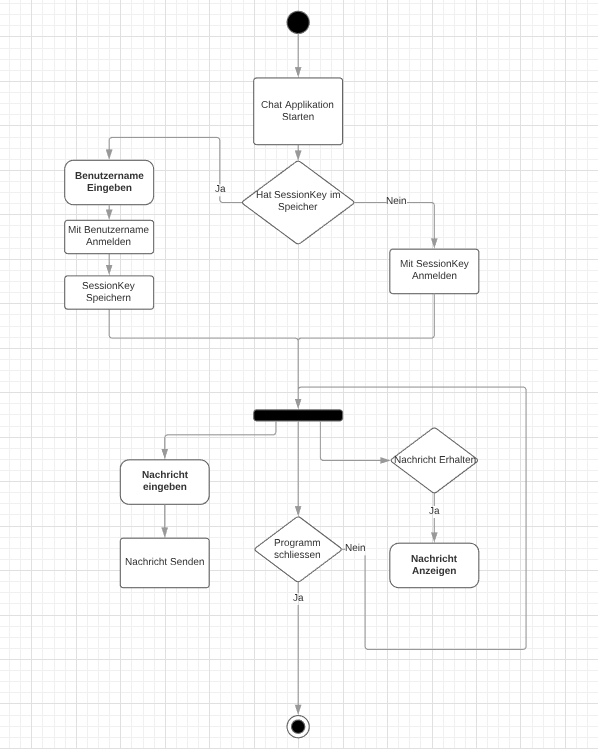
\includegraphics[height=0.9\textheight]{activity-diagram.png}}
      \subsubsection{USER\_LOGIN\_STANDARD Use Case}
        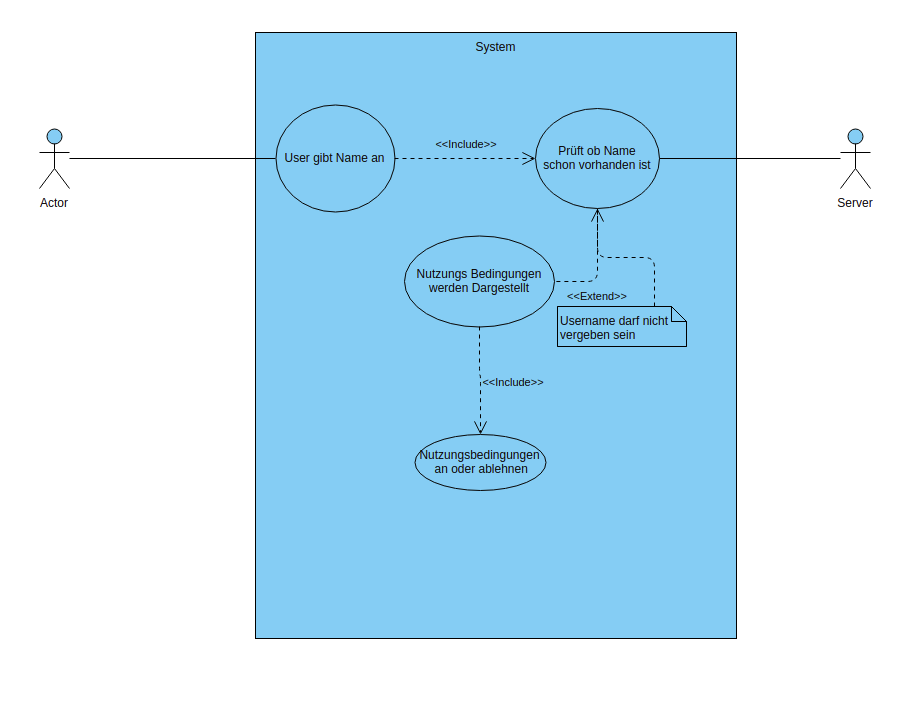
\includegraphics[width=\textwidth]{useCase_USER_LOGIN_STANDARD.png}

    \subsection{Zielsetzungen}
      \subsubsection{Muss-Ziele}
        \begin{enumerate}
          \item \faGlobe~   Globaler Gruppen Chat
          \item \faUser~    Hinterlegen eines Benutzernamens
          \item \faKey~     Benutzer muss den Chat später wieder aufnehmen können. z.B. cookies oder Session Storage
          \item \faMobile~  Die Seite für Mobile geräte optimieren
        \end{enumerate}

      \subsubsection{Kann-Ziele}
        \begin{enumerate}
          \item \faUsers~   Private Chats zwischen zwei Personen
          \item \faGoogle~  Authentifizierung über Google Accounts aber trotzdem anonyme
        \end{enumerate}

    \subsection{Akteure}
        \begin{table}[H]
          \begin{tabularx}{\textwidth}{|l|X|}
            \hline
            Nicht Angemeldeter Benutzer & Hat nur die Berechtigung, sich anzumelden  \\ \hline
            Angemeldeter Benutzer & Kann Nachrichten verschicken und erhalten  \\ \hline
            Administrator & Hat Zugriff auf Verwaltungsinformationen und auf die Datenbank \\ \hline
          \end{tabularx}
        \end{table}


    \subsection{Funktionale Anforderungen}
      \subsubsection{Anforderungen aus der Sicht des unprivilegierten Benutzers}
        \requirementTable
            {USER\_LOGIN\_STANDARD}
            {Nicht Angemeldeter Benutzer}
            {Macht die Applikation das erste mal auf}
            {
            Er gibt seinen gewünschten Namen ein. \newline
            Es wird geprüft, ob es jemanden mit dem Namen schon gibt. \newline
            Dann erscheint ein Popup mit den Nutzungsbedingungen. Der Benutzer kann nun Annehmen oder Abbrechen auswählen
            }
            {
            Falls der Benutzer die Nutzungsbedingungen akzeptiert, ist er auf der Chatseite und ist auf dem Server authentifiziert. Falls der Benutzer die Nutzungsbedingungen abgelehnt hat, ist er wieder im Ausgangsbildschirm.
            }

        \requirementTable
            {USER\_LOGIN\_GOOGLE}
            {Nicht Angemeldeter Benutzer}
            {Macht die Applikation das erste mal auf}
            {
            Er klickt auf die Option “mit Google anmelden” \newline
            Die Authentifizierung über Google erfolgt. \newline
            Falls die Anmeldung gültig ist, dann erscheint ein Popup mit den Nutzungsbedingungen. Der Benutzer kann nun Annehmen oder Abbrechen auswählen. \newline
            Falls keine gültige Anmeldung über Google erfolgt, wird der Anmeldeprozess wieder auf den Start gestellt.
            }
            {
            Falls der Benutzer sich mit Google korrekt authentifiziert hat und  die Nutzungsbedingungen akzeptiert, ist er auf der Chatseite und ist auf dem Server authentifiziert. \newline
            Falls der Benutzer sich nicht via Google anmelden konnte oder er die Nutzungsbedingungen abgelehnt hat, ist er wieder im Ausgangsbildschirm.
            }

        \requirementTable
            {NACHRICHT\_SENDEN}
            {Angemeldeter Benutzer}
            {Ist bereits angemeldet und auf der Chatseite}
            {Gibt eine Nachricht ein und sendet diese ab}
            {Die Nachricht kommt beim Server an und wird and die verschiedenen Benutzer gesendet und angezeigt.}

        \requirementTable
            {NACHRICHT\_EMPFAGEN}
            {Angemeldeter Benutzer}
            {Ist bereits angemeldet und auf der Chatseite}
            {Bekommt eine Nachricht vom Server}
            {Die Nachricht wird auf der Applikation angezeigt}


        \requirementTable
            {PRIVATER\_CHAT\_ANFRAGE}
            {Angemeldeter Benutzer}
            {
            Benutzer ist bereits angemeldet und auf der Chatseite. \newline
            Es ist ein zweiter Benutzer ebenfalls im Chat angemeldet
            }
            {
            Der Benutzer 1 macht einen Rechtsklick auf den zweiten Benutzer. \newline
            Es erscheint ein Dialog, ob er einen Privatchat starten will. \newline
            Falls er das bestätigt, erscheint beim zweiten Benutzer eine Meldung, dass Benutzer 1 ihn zu einem Privatchat eingeladen hat.
            }
            {Meldung an zweiten Benutzer verschickt mit der Anfrage für einen Privatchat.}


        \requirementTable
            {PRIVATER\_CHAT\_ERSTELLEN\_PERSON\_\newline NIMMT\_AN }
            {Angemeldeter Benutzer}
            {
            Ist bereits angemeldet und auf der Chatseite. \newline
            Hat von einem anderen Benutzer eine Anfrage für einen Privatchat erhalten.}
            {
            Der Benutzer macht einen Rechtsklick auf die Meldung Im Dialog klickt er auf “Zum Privaten Chat wechseln”. \newline
            Der anfragende Benutzer erhält eine Meldung, dass der Benutzer zu seinem Privatchat gewechselt hat
            }
            {Der Benutzer und der anfragende Benutzer sind in einem Privatchat}


        \requirementTable
            {PRIVATER\_CHAT\_ERSTELLEN\_PERSON\_\newline LEHNT\_AB}
            {Angemeldeter Benutzer}
            {
            Ist bereits angemeldet und auf der Chatseite. \newline
            Hat von einem anderen Benutzer eine Anfrage für einen Privatchat erhalten
            }
            {
            Der Benutzer macht einen Rechtsklick auf die Meldung Im Dialog klickt er auf “Nicht zum Privaten Chat wechseln”\newline
            oder er ignoriert die Anfrage
            }
            {
            Der Benutzer bleibt im normalen Chat. \newline
            Beim anfragenden Benutzer erscheint die Meldung, dass kein Privatchat zustande gekommen ist.
            }


      \subsubsection{Anforderungen aus der Sicht der privilegierten Benutzer}
        \requirementTable
            {BENUTZER\_AUS\_CHAT\_ENTFERNEN}
            {Admin}
            {
            ist als Administrator angemeldet. \newline
            Ein momentan angemeldeter Benutzer verstösst im laufenden Chat gegen die Vorgaben des Chats.
            }
            {
            Falls ein Benutzer sich nicht an die Vorgaben hält, kann er aus dem Chat durch einen Administrator entfernt werden, indem sein Token gelöscht wird. \newline
            Im Chat erfolgt eine generierte Nachricht, “Benutzer xxx aus Chat entfernt”
            }
            {Der Benutzer ist nicht mehr im Chat angemeldet}


        \requirementTable
            {CHAT\_HISTORIE\_AUS\_CHAT\_ENTFERNEN}
            {Admin}
            {
            ist als Administrator angemeldet. \newline
            Ein  Benutzer hat gegen die Vorgaben des Chats verstossen und seine Einträge müssen entfernt werden. Es ist egal, ob der Benutzer angemeldet ist oder nicht.
            }
            {
            Der Administrator kann jederzeit, auch wenn der Benutzer nicht mehr angemeldet ist, die ganze Historie der Chats dieses Benutzer löschen.
            }
            {
            Die Chatnachrichten des jeweiligen Benutzers werden für alle gelöscht.
            }

      \subsubsection{Anforderungen aus der Sicht des Systems}
         \requirementTable
            {UPDATEN}
            {System}
            {Ist nicht zum ersten mal auf der Applikation}
            {Schaut ob eine neue Version verfügbar ist und aktualisiert zur neuesten Version.}
            {Ist auf der neusten Version der Applikation.}

    \section{Mockups}
        \subsection{Android frame}
        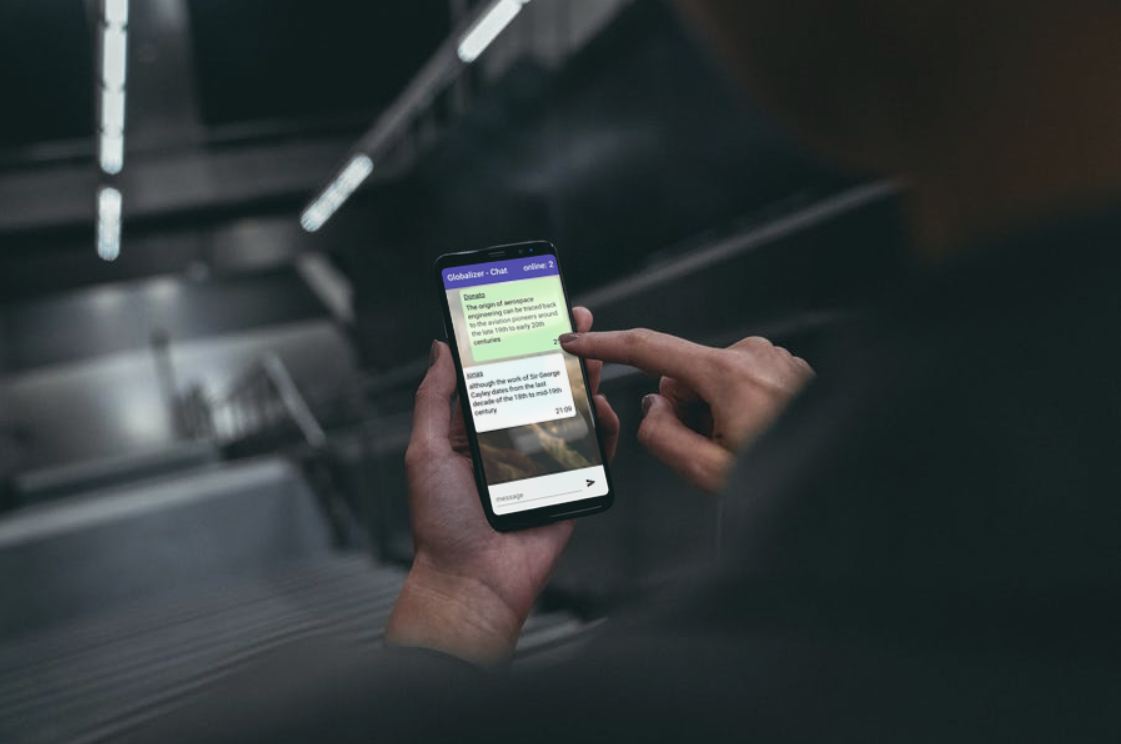
\includegraphics[width=\textwidth]{mock-chat.png}
        \subsection{Desktop Chrome Login}
        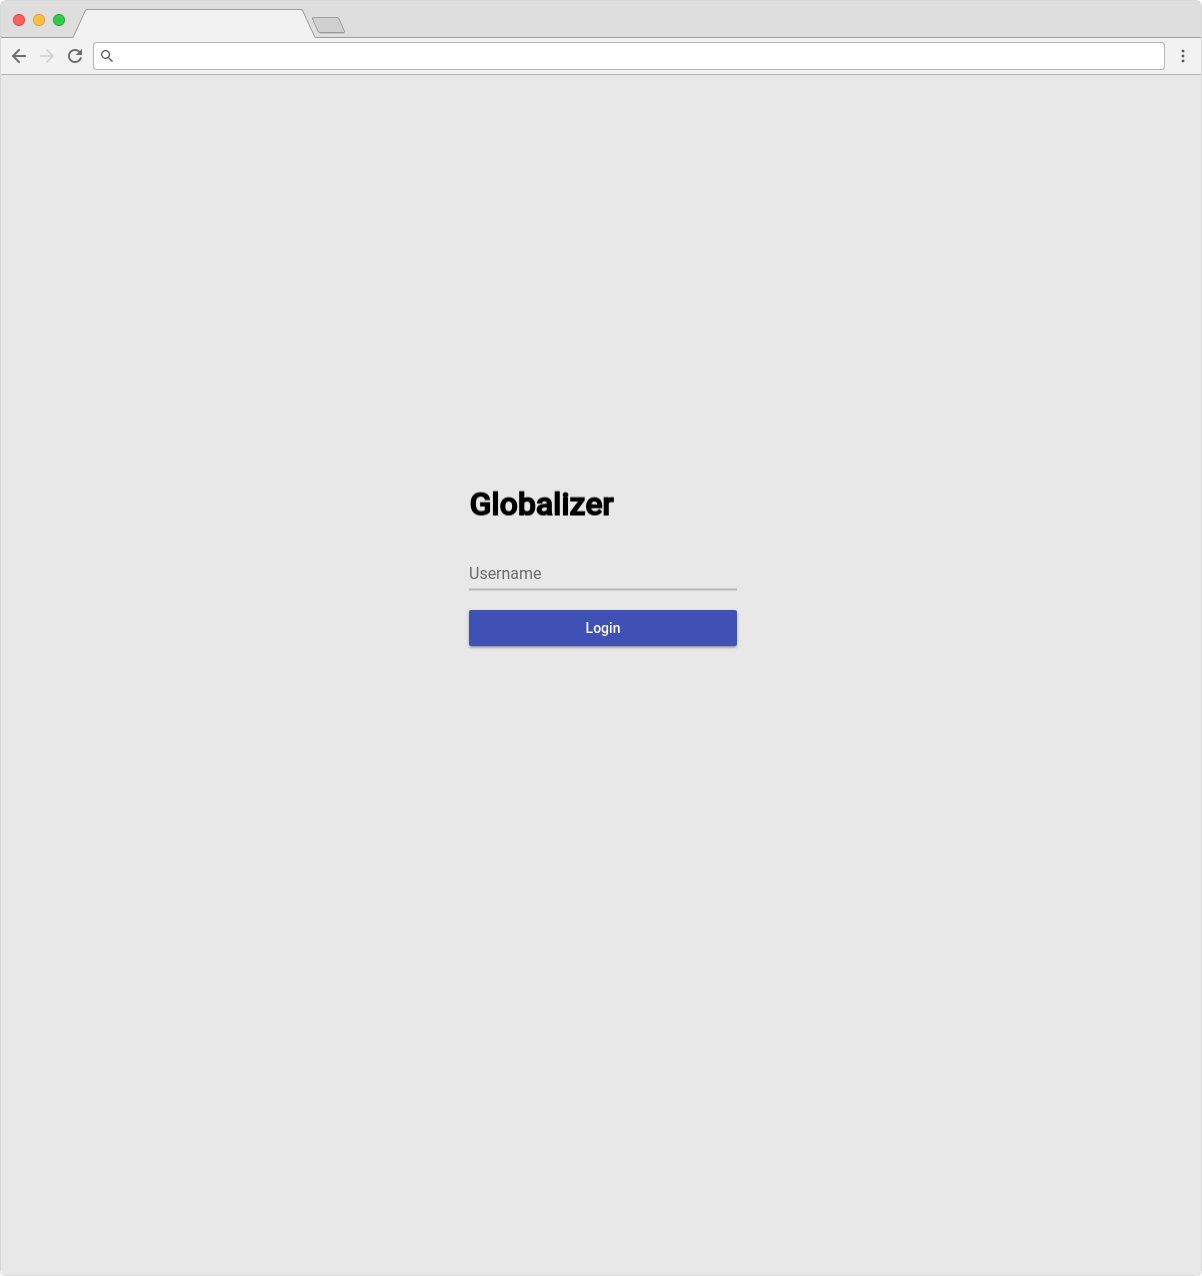
\includegraphics[width=\textwidth]{frame-desktop-login.png}

        \subsection{Desktop Chrome Chat}
        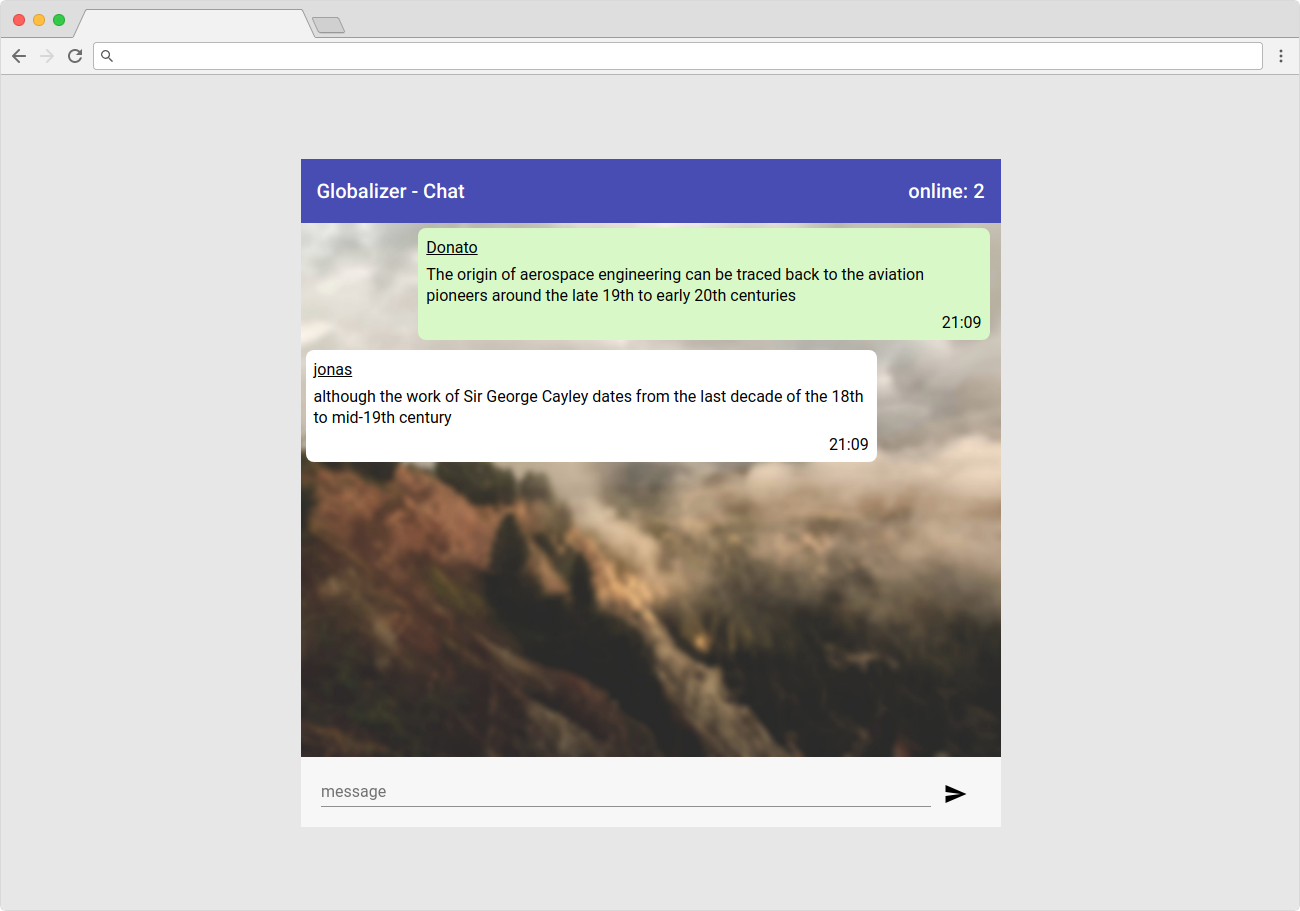
\includegraphics[width=\textwidth]{frame-desktop-chat.png}
\end{document}
